\documentclass{standalone}

\begin{document}

\subsection[Results]{Results}\label{obj_detection:results}

The original implementation of the YOLO model was provided by Redmon et al. and it is publicly available in his official \href{https://pjreddie.com/darknet/yolo}{web page} of the \textsf{darknet} project.
The code is written in \textsf{Ansi-C} and it is designed and, only thank to the many branches developed by the Github community, it can be compiled on all the OS.
The \textsf{Ansi-C} language is a very low-level programming language and it is hard to obtain better performances rewriting the code.
This guarantees its supremacy in terms of speed in the research community.
The code is particularly optimized for GPU applications: the \textsf{darknet} library provides an efficient CUDA support and it can be optimally used only with NVIDIA GPUs.

The proposed \textsf{Byron} library has been developed following the backbone and innovative ideas provided by the \textsf{darknet} project.
The main difference between them is the programming language chosen: \textsf{Byron} is written in pure \textsf{C++}, a \quotes{higher}-level programming language.
Generally, we can not obtain better computational performances using \textsf{C++} in relation to an \textsf{Ansi-C} implementation.
However, the \textsf{C++} language is more popular than \textsf{Ansi-C} and more easy to write and modify.
The second main difference of \textsf{Byron} is related to the target computational environment: it is designed and optimized to reach the better performances on a single or multiple CPUs architecture.
In this way we aim to enlarge also the usability of our code.
Many research groups, in fact, have very powerful server grade machines, without a GPU support and it is hard for them to get close to the deep learning applications.
An emblematic case is given by the bioinformatics research, in which a large amount of money are spent to buy efficient server grade machines to process large DNA datasets which are commonly processed using only CPUs support.

In the previous sections we have discussed about different kinds of optimization related to the various (possible) components of a Neural Network model.
All these optimizations were implemented in the \textsf{Byron} library to reach the best performances.
Moreover, studying the Redmon et al. implementation, many issues were found in the \textsf{darknet} project, especially related to the multi-threading support and thread concurrency.
\textsf{Byron} library widely uses OpenMP features, paying attention to thread concurrencies, minimizing the time for thread spawning.
In \textsf{Byron} a single parallel section is open at the beginning of the processing and it is closed at the end, with a carefully management of the threads along all the network structure.

In view of these considerations, a first test was performed to compare the \textsf{Byron} efficiency against the \textsf{darknet} one, in terms of time-performances.
To compare the results, we implemented the same YOLO model into our custom \textsf{Byron} framework and we compared its time efficiency against the original implementation.
Tests were performed turning off the multi-threading support, since the \textsf{darknet} implementation uses it only in the \textsf{GEMM} steps.
We performed $5$ independent simulations using the same input image to test the time stability of both implementations.
Each simulation performed $100$ runs of both algorithms.
The results are shown in Fig.~\ref{fig:yolo_time}, where we have normalized our times in relation to the \textsf{darknet} ones (reference).

\begin{figure}[htbp]
\centering
\def\svgwidth{0.85\textwidth}
\input{./img/byron_timing.pdf_tex}
\caption{Comparison of time performances between the \textsf{Byron} and \textsf{darknet} implementations of YOLO model.
Simulations were performed keeping fixed the input image sizes and wit any multi-threading support.
Each simulation includes $100$ runs of both algorithms.
The \textsf{Byron} version is approximately $3.8$x faster than \textsf{darknet} in all the simulations.
}
\label{fig:yolo_time}
\end{figure}

Both implementations are quite stable across the simulations and our measures show a very tight variability.
The differences in time performances are evident and we can summarize them with a $3.8$x speedup obtained by \textsf{Byron} against \textsf{darknet}.
The multiple optimizations discussed and used by \textsf{Byron} are proved by numerical results and they highlight the efficiency of our implementation against the state-of-art.
We would stress that, using our version of the model into a server grade machine (128~GB RAM memory and 2 CPU E5-2620, with 8 cores each), YOLO can process $416\times416$ images in real-time (less than a second), while \textsf{darknet} can reach the same performances only with a GPU support.

Once the efficiency has been proved, we \quotes{update} the YOLO model to overcome its issues.
In particular, we have discussed in the previous section (ref. \ref{obj_detection:yolo}) that the biggest issue related to YOLO concerns the detection of small objects.
Despite the model is incredibly efficient in object detection also with low quality images, there is a sort of limit in the number of pixels needed for object identification.
This kind of problems are particularly critical in people counting tasks, and moreover in crowd counting applications.
YOLO is able to identify the major part of persons into an image, but it decreases its efficiency when they partly overlap or they are far from the camera (and thus at low resolution).

We had the opportunity to empirically verify its limit, working on a people tracking project for real-time applications.
The project was developed in collaboration with the Complex Systems (\emph{PhySyCom}) group of the University of Bologna, with the support of Canon Inc., Telecom Italia and Fabbrica Digitale, and it aims to detect and track people, using video camera devices.
The experiments were executed around the streets of Venice city, with the support of the Venice City Council.
Using our custom implementation of YOLO we were able to detect the major part of persons, but we lost efficiency when the people flow increased or when we face with open space area (a crucial point was Piazza San Marco).

In the previous section we have largely discussed about the efficiency of Super Resolution techniques to improve the image quality, so it stands to reason that their application will be helpful to overcome the told above issue.
We applied the previously described EDSR model to critical images, i.e where YOLO did not perfectly detect all the people in the picture.
For privacy reasons, we can not show the results obtained on Venice data, but we can show a simple example to prove our combination of models.
The example is shown in Fig.~\ref{fig:yolo_sr}.

\begin{figure}[htbp]
\centering
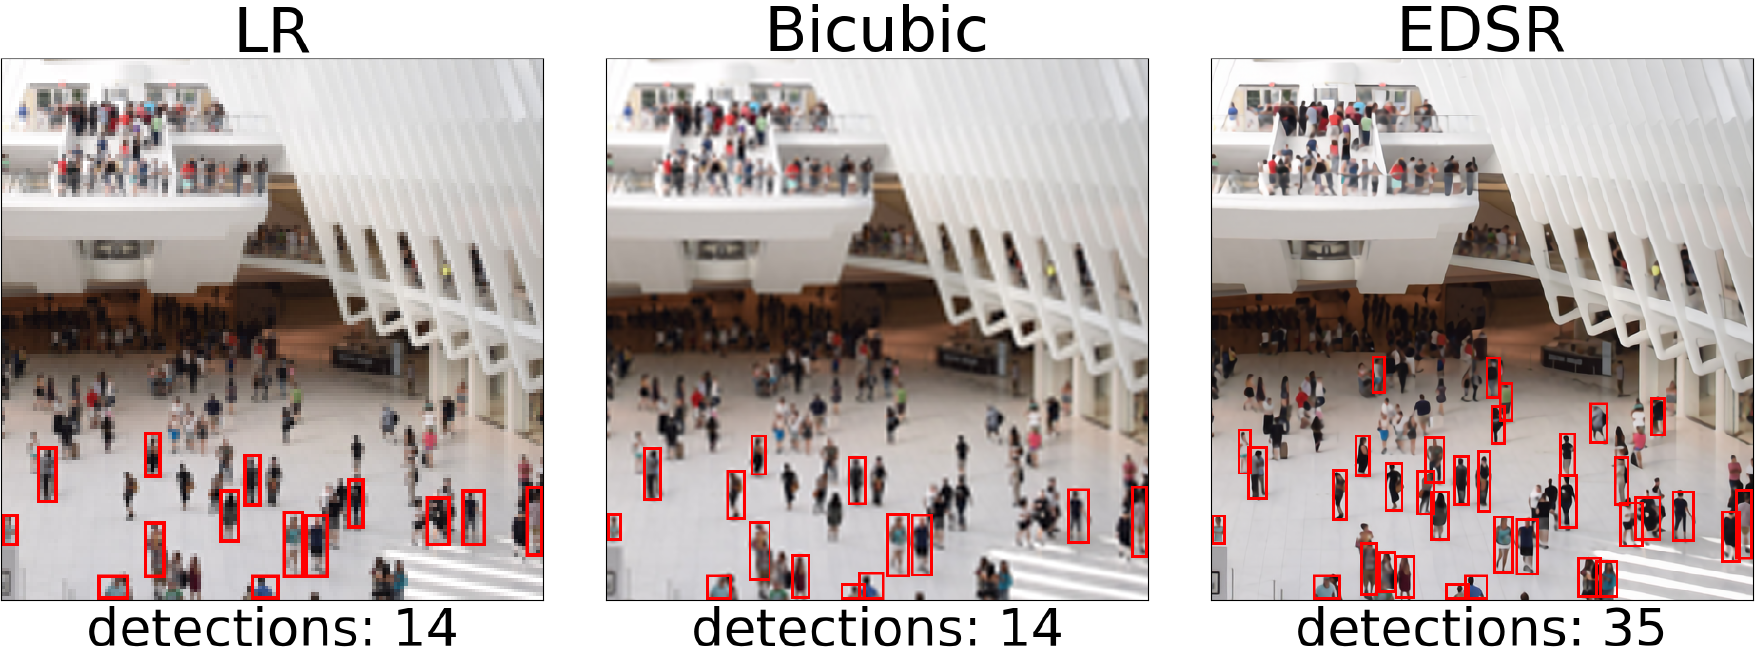
\includegraphics[width=0.85\textwidth]{yolo_people_sr.png}
\caption{YOLO people detections on a image ROI.
\textbf{(left)} The original ROI and its corresponding detections.
\textbf{(center)} Up-sampling of the original ROI using a bi-cubic algorithm and its corresponding detections.
\textbf{(right)} Up-sampling of the original ROI using the EDSR model and its corresponding detections.
The use of Super Resolution model is able to improve the YOLO detection of small persons of more than 200\%.
YOLO is not still able to detect the smaller (far) persons.
}
\label{fig:yolo_sr}
\end{figure}

On the first image (left of Fig.~\ref{fig:yolo_sr}) we show only a small ROI of a (larger) input image, where YOLO is able to find only few people.
We would remark that the detected people are all in the bottom part of the image, where person \quotes{sizes} are bigger.
Using a standard bicubic up-sampling (center of Fig.~\ref{fig:yolo_sr}) detection performances are the same, proving as standard up-sampling methods are not appropriate to overcome this task.
The application of EDSR model (right of Fig.~\ref{fig:yolo_sr}) is able to improve the quality of the image and ease the YOLO work.
In this case the detection is more than twice of the previous case.
The issue remains for the top part of the image, where only few pixels identify a person.
Set out to test the limit of this model combination, we have extracted a further ROI from it, selecting only the top part of the image.
The results are shown in Fig.~\ref{fig:yolo_sr2}.

\begin{figure}[htbp]
\centering
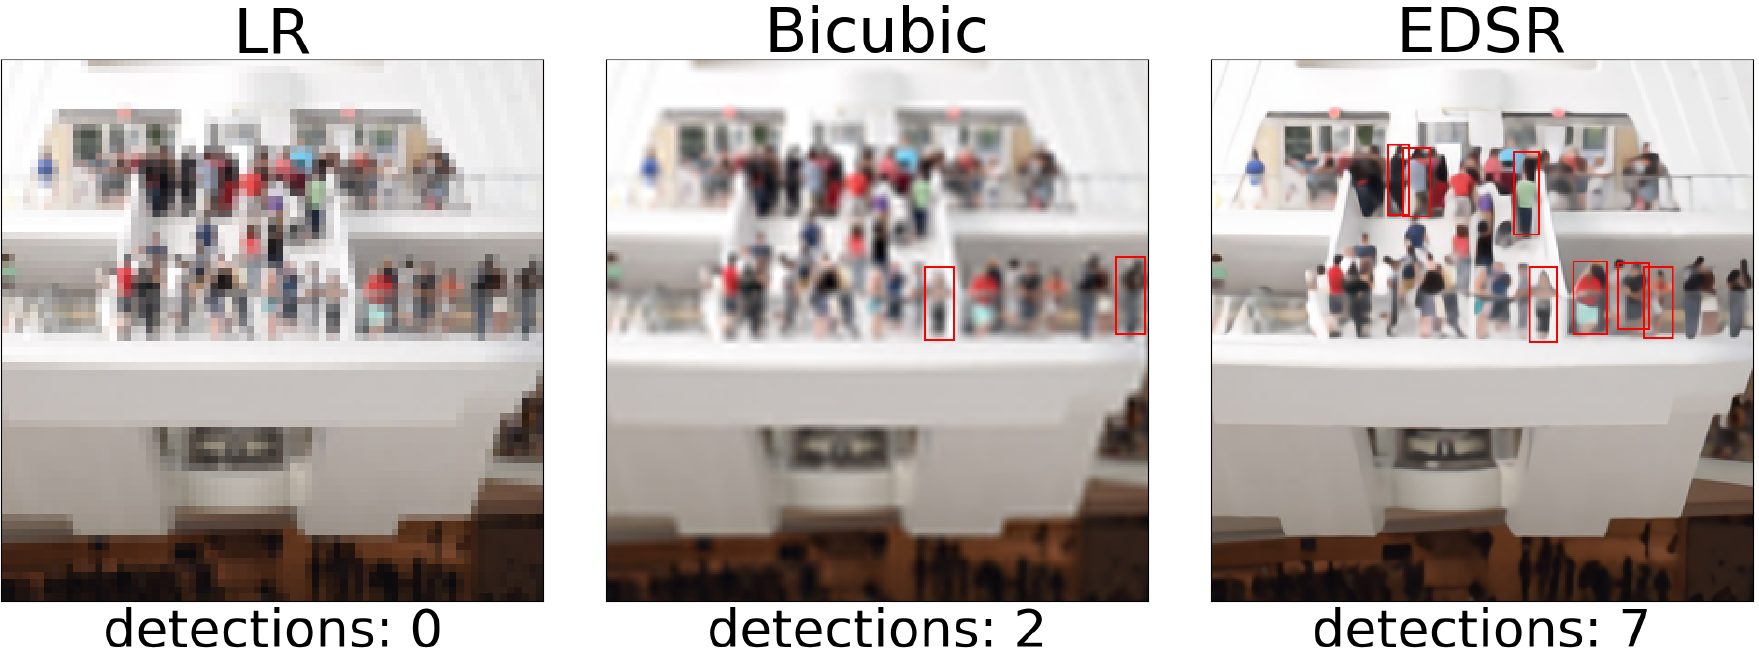
\includegraphics[width=0.85\textwidth]{yolo_people_sr2.png}
\caption{YOLO people detections on a ROI of the previous image ROI.
\textbf{(left)} The original ROI and its corresponding detections.
\textbf{(center)} Up-sampling of the original ROI using a bi-cubic algorithm and its corresponding detections.
\textbf{(right)} Up-sampling of the original ROI using the EDSR model and its corresponding detections.
Without the Super Resolution application the YOLO model is not able to recognize any person.
The bi-cubic up-sampling allows the detection of only 2 persons against the 7 obtained by the use of EDSR model.
}
\label{fig:yolo_sr2}
\end{figure}

The task in this case is certainly harder and also human eyes hardly count the number of persons into the image.
With the raw image, YOLO is able to find anything and also with the bicubic up-sampling only 1 person is recognized by the model.
With the EDSR pre-processing, the detection performance increases and $7$ persons are recognized.
Certainly, the people count is underestimated, but Super Resolution pre-processing seems to be the only available solution to improve YOLO performances on these critical cases.


\end{document}
